\documentclass[journal,12pt,twocolumn]{IEEEtran}
%
\usepackage{setspace}
\usepackage{gensymb}
%\doublespacing
\singlespacing

%\usepackage{graphicx}
%\usepackage{amssymb}
%\usepackage{relsize}
\usepackage[cmex10]{amsmath}
%\usepackage{amsthm}
%\interdisplaylinepenalty=2500
%\savesymbol{iint}
%\usepackage{txfonts}
%\restoresymbol{TXF}{iint}
%\usepackage{wasysym}
\usepackage{amsthm}
%\usepackage{iithtlc}
\usepackage{mathrsfs}
\usepackage{txfonts}
\usepackage{stfloats}
\usepackage{bm}
\usepackage{cite}
\usepackage{cases}
\usepackage{subfig}
%\usepackage{xtab}
\usepackage{longtable}
\usepackage{multirow}
%\usepackage{algorithm}
%\usepackage{algpseudocode}
\usepackage{enumitem}
\usepackage{mathtools}
\usepackage{tikz}
\usepackage{circuitikz}
\usepackage{verbatim}
%\usepackage{tfrupee}
\usepackage[breaklinks=true]{hyperref}
%\usepackage{stmaryrd}
\usepackage{tkz-euclide} % loads  TikZ and tkz-base
%\usetkzobj{all}
\usepackage{listings}
    \usepackage{color}                                            %%
    \usepackage{array}                                            %%
    \usepackage{longtable}                                        %%
    \usepackage{calc}                                             %%
    \usepackage{multirow}                                         %%
    \usepackage{hhline}                                           %%
    \usepackage{ifthen}                                           %%
  %optionally (for landscape tables embedded in another document): %%
    \usepackage{lscape}     
\usepackage{multicol}
\usepackage{chngcntr}
%\usepackage{enumerate}

%\usepackage{wasysym}
%\newcounter{MYtempeqncnt}
\DeclareMathOperator*{\Res}{Res}
%\renewcommand{\baselinestretch}{2}
\renewcommand\thesection{\arabic{section}}
\renewcommand\thesubsection{\thesection.\arabic{subsection}}
\renewcommand\thesubsubsection{\thesubsection.\arabic{subsubsection}}

\renewcommand\thesectiondis{\arabic{section}}
\renewcommand\thesubsectiondis{\thesectiondis.\arabic{subsection}}
\renewcommand\thesubsubsectiondis{\thesubsectiondis.\arabic{subsubsection}}

% correct bad hyphenation here
\hyphenation{op-tical net-works semi-conduc-tor}
\def\inputGnumericTable{}                                 %%

\lstset{
%language=C,
frame=single, 
breaklines=true,
columns=fullflexible
}
%\lstset{
%language=tex,
%frame=single, 
%breaklines=true
%}

\begin{document}

\newtheorem{theorem}{Theorem}[section]
\newtheorem{problem}{Problem}
\newtheorem{proposition}{Proposition}[section]
\newtheorem{lemma}{Lemma}[section]
\newtheorem{corollary}[theorem]{Corollary}
\newtheorem{example}{Example}[section]
\newtheorem{definition}[problem]{Definition}
%\newtheorem{thm}{Theorem}[section] 
%\newtheorem{defn}[thm]{Definition}
%\newtheorem{algorithm}{Algorithm}[section]
%\newtheorem{cor}{Corollary}
\newcommand{\BEQA}{\begin{eqnarray}}
\newcommand{\EEQA}{\end{eqnarray}}
\newcommand{\define}{\stackrel{\triangle}{=}}
\bibliographystyle{IEEEtran}
%\bibliographystyle{ieeetr}
\providecommand{\mbf}{\mathbf}
\providecommand{\pr}[1]{\ensuremath{\Pr\left(#1\right)}}
\providecommand{\qfunc}[1]{\ensuremath{Q\left(#1\right)}}
\providecommand{\sbrak}[1]{\ensuremath{{}\left[#1\right]}}
\providecommand{\lsbrak}[1]{\ensuremath{{}\left[#1\right.}}
\providecommand{\rsbrak}[1]{\ensuremath{{}\left.#1\right]}}
\providecommand{\brak}[1]{\ensuremath{\left(#1\right)}}
\providecommand{\lbrak}[1]{\ensuremath{\left(#1\right.}}
\providecommand{\rbrak}[1]{\ensuremath{\left.#1\right)}}
\providecommand{\cbrak}[1]{\ensuremath{\left\{#1\right\}}}
\providecommand{\lcbrak}[1]{\ensuremath{\left\{#1\right.}}
\providecommand{\rcbrak}[1]{\ensuremath{\left.#1\right\}}}
\theoremstyle{remark}
\newtheorem{rem}{Remark}
\newcommand{\sgn}{\mathop{\mathrm{sgn}}}
\providecommand{\abs}[1]{\left\vert#1\right\vert}
\providecommand{\res}[1]{\Res\displaylimits_{#1}} 
\providecommand{\norm}[1]{\left\lVert#1\right\rVert}
%\providecommand{\norm}[1]{\lVert#1\rVert}
\providecommand{\mtx}[1]{\mathbf{#1}}
\providecommand{\mean}[1]{E\left[ #1 \right]}
\providecommand{\fourier}{\overset{\mathcal{F}}{ \rightleftharpoons}}
%\providecommand{\hilbert}{\overset{\mathcal{H}}{ \rightleftharpoons}}
\providecommand{\system}{\overset{\mathcal{H}}{ \longleftrightarrow}}
	%\newcommand{\solution}[2]{\textbf{Solution:}{#1}}
\newcommand{\solution}{\noindent \textbf{Solution: }}
\newcommand{\cosec}{\,\text{cosec}\,}
\providecommand{\dec}[2]{\ensuremath{\overset{#1}{\underset{#2}{\gtrless}}}}
\newcommand{\myvec}[1]{\ensuremath{\begin{pmatrix}#1\end{pmatrix}}}
\newcommand{\mydet}[1]{\ensuremath{\begin{vmatrix}#1\end{vmatrix}}}
%\numberwithin{equation}{section}
%\numberwithin{equation}{subsection}
%\numberwithin{problem}{section}
%\numberwithin{definition}{section}
\makeatletter
\@addtoreset{figure}{problem}
\makeatother
\let\StandardTheFigure\thefigure
\let\vec\mathbf
%\renewcommand{\thefigure}{\theproblem.\arabic{figure}}
\renewcommand{\thefigure}{\theproblem}
%\setlist[enumerate,1]{before=\renewcommand\theequation{\theenumi.\arabic{equation}}
%\counterwithin{equation}{enumi}
%\renewcommand{\theequation}{\arabic{subsection}.\arabic{equation}}
\def\putbox#1#2#3{\makebox[0in][l]{\makebox[#1][l]{}\raisebox{\baselineskip}[0in][0in]{\raisebox{#2}[0in][0in]{#3}}}}
     \def\rightbox#1{\makebox[0in][r]{#1}}
     \def\centbox#1{\makebox[0in]{#1}}
     \def\topbox#1{\raisebox{-\baselineskip}[0in][0in]{#1}}
     \def\midbox#1{\raisebox{-0.5\baselineskip}[0in][0in]{#1}}
\vspace{3cm}
\title{
%	\logo{
MATHEMATICS
%	}
}
\author{ G V V Sharma$^{*}$% <-this % stops a space
	\thanks{*The author is with the Department
		of Electrical Engineering, Indian Institute of Technology, Hyderabad
		502285 India e-mail:  gadepall@iith.ac.in. All content in this manual is released under GNU GPL.  Free and open source.}
	
}	
%\title{
%	\logo{Matrix Analysis through Octave}{\begin{center}\includegraphics[scale=.24]{tlc}\end{center}}{}{HAMDSP}
%}
% paper title
% can use linebreaks \\ within to get better formatting as desired
%\title{Matrix Analysis through Octave}
%
%
% author names and IEEE memberships
% note positions of commas and nonbreaking spaces ( ~ ) LaTeX will not break
% a structure at a ~ so this keeps an author's name from being broken across
% two lines.
% use \thanks{} to gain access to the first footnote area
% a separate \thanks must be used for each paragraph as LaTeX2e's \thanks
% was not built to handle multiple paragraphs
%
%\author{<-this % stops a space
%\thanks{}}
%}
% note the % following the last \IEEEmembership and also \thanks - 
% these prevent an unwanted space from occurring between the last author name
% and the end of the author line. i.e., if you had this:
% 
% \author{....lastname \thanks{...} \thanks{...} }
%                     ^------------^------------^----Do not want these spaces!
%
% a space would be appended to the last name and could cause every name on that
% line to be shifted left slightly. This is one of those "LaTeX things". For
% instance, "\textbf{A} \textbf{B}" will typeset as "A B" not "AB". To get
% "AB" then you have to do: "\textbf{A}\textbf{B}"
% \thanks is no different in this regard, so shield the last } of each \thanks
% that ends a line with a % and do not let a space in before the next \thanks.
% Spaces after \IEEEmembership other than the last one are OK (and needed) as
% you are supposed to have spaces between the names. For what it is worth,
% this is a minor point as most people would not even notice if the said evil
% space somehow managed to creep in.
% The paper headers
%\markboth{Journal of \LaTeX\ Class Files,~Vol.~6, No.~1, January~2007}%
%{Shell \MakeLowercase{\textit{et al.}}: Bare Demo of IEEEtran.cls for Journals}
% The only time the second header will appear is for the odd numbered pages
% after the title page when using the twoside option.
% 
% *** Note that you probably will NOT want to include the author's ***
% *** name in the headers of peer review papers.                   ***
% You can use \ifCLASSOPTIONpeerreview for conditional compilation here if
% you desire.
% If you want to put a publisher's ID mark on the page you can do it like
% this:
%\IEEEpubid{0000--0000/00\$00.00~\copyright~2007 IEEE}
% Remember, if you use this you must call \IEEEpubidadjcol in the second
% column for its text to clear the IEEEpubid mark.
% make the title area


\maketitle
\newpage
%\tableofcontents
\bigskip
\renewcommand{\thefigure}{\theenumi}
\renewcommand{\thetable}{\theenumi}
%\renewcommand{\theequation}{\theenumi}
%\begin{abstract}
%%\boldmath
%In this letter, an algorithm for evaluating the exact analytical bit error rate  (BER)  for the piecewise linear (PL) combiner for  multiple relays is presented. Previous results were available only for upto three relays. The algorithm is unique in the sense that  the actual mathematical expressions, that are prohibitively large, need not be explicitly obtained. The diversity gain due to multiple relays is shown through plots of the analytical BER, well supported by simulations. 
%
%\end{abstract}
% IEEEtran.cls defaults to using nonbold math in the Abstract.
% This preserves the distinction between vectors and scalars. However,
% if the journal you are submitting to favors bold math in the abstract,
% then you can use LaTeX's standard command \boldmath at the very start
% of the abstract to achieve this. Many IEEE journals frown on math
% in the abstract anyway.
% Note that keywords are not normally used for peerreview papers.
%\begin{IEEEkeywords}
%Cooperative diversity, decode and forward, piecewise linear
%\end{IEEEkeywords}
% For peer review papers, you can put extra information on the cover
% page as needed:
% \ifCLASSOPTIONpeerreview
% \begin{center} \bfseries EDICS Category: 3-BBND \end{center}
% \fi
%
% For peerreview papers, this IEEEtran command inserts a page break and
% creates the second title. It will be ignored for other modes.
%\IEEEpeerreviewmaketitle
%\begin{abstract}
%This manual includes \LaTeX figures.
%book provides an introduction to optimization  based on the NCERT textbooks from Class 6-12.  Links to sample Python codes are available in the text.  
%\end{abstract}
Download 
\begin{lstlisting}
https://github.com/RaghavendraKulkarni6398/QuestionPaper2010
\end{lstlisting}

\begin{document}
\vspace{0.15in}
\begin{center}
\parbox{1in}{
{\textsc{\textbf{Section A} }}}}
\end{center}
\vspace{0.15in}
\hrule 
\vspace{0.1in}
\begin{enumerate}

\item 1. Write whether $\frac{2\sqrt{45}+3\sqrt{20}}{2\sqrt{5}} $ on simplification gives a rational or an irrational number \\
\vspace{0.2in}
\item If $\alpha,\beta$ are the zeroes of the polynomial $2y^2 + 7y + 5$, write the value of $\alpha + \beta + \alpha\beta$.
\vspace{0.2in}
\item If the sum of the first q terms of an A.P is $ 2q + 3q^2 $ what is its common difference?
\vspace{0.2in}
\item In Figure 1, CP and CQ are tangents from an external point C to a circle with centre O. AB are another
\vspace{0.2in}
tangent which touches the circle at R. If CP = 11 cm and BR = 4 cm, find the length of BC.
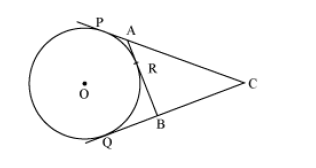
\includegraphics[width=\columnwidth]{fig1.png}
\vspace{0.2in}
\item In Figure 2, DE$| |$BC in ABC such that BC = 8 cm, AB = 6 cm and DA = 1.5 cm. Find DE.
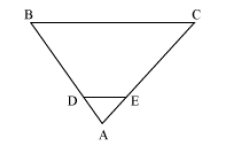
\includegraphics[width=\columnwidth, height=5cm]{fig2.png}
\vspace{0.2in}
\item  If $ 5x=sec\theta $ and $\left\frac{5}{x}=tan\theta\right$ find the value of $5(x^2 - \frac{1}{x^2}$) 
\vspace{0.2in}
\item What is the distance between the points A (c, 0) and B(0, –c)?
\vspace{0.2in}
\item  In a $\triangle ABC $, right-angled at C, AC = 6 cm and AB = 12 cm. Find $\angle$ A.
 
\item  The slant height of the frustum of a cone is 5 cm. If the difference between the radii of its two circular
ends is 4 cm, write the height of the frustum.
\vspace{0.3in}
\item  A die is thrown once. What is the probability of getting a number greater than 4?
 \vspace{0.3in} 
\item  For what value of k, is 3 a zero of the polynomial 2x2 + x + k?
\vspace{0.3in}      
\item  Find the value of m for which the pair of linear equations 2x + 3y – 7 = 0 and (m – 1) x + (m + 1) y =
(3m – 1) has infinitely many solutions.
\vspace{0.3in}    
\item  Find the common difference of an A.P. whose first term is 4, the last term is 49 and the sum of all its
terms is 265.
\vspace{0.3in} 
\item In figure 3, there are two concentric circles with centre O and of radii 5 cm and 3 cm. From an
external point P, Tangents PA and PB are drawn to these circles. If AP = 12 cm, find the length of BP.
\vspace{0.3in}
\item  Without using trigonometric tables, evaluate the following:
$\frac{cos 70\degree}{3 sin 20\degree}$ + $ \frac{4(sec^2 59\degree - cot^231\degree}{3} $ - $\frac{2}{3}sin 90\degree$
   
\vspace{0.3in}

\item  Solve the following pair of linear equations for x and y:
 \vspace{0.3in} 
\item Solve the following pair of linear equations for x and y: $\frac{b}{a}x + \frac{a}{b}y = a^2+b^2$ and $ x+y = 2ab $
    \vspace{0.3in} 
 \item  In an A.P., the sum of its first ten terms is – 80 and the sum of its next ten terms is – 280. Find the
A.P.
 
\vspace{0.3in} 
\item  In figure 4, ABC is an isosceles triangle in which AB = AC. E is a point on the side CB produced,
such that $FE \perp AC$. If $AD \perp CB$, prove that:
AB$\times$ EF = AD $\times$ EC

 \vspace{0.3in}
 
\item  Prove the following:$ (1+cotA - cosec A)(1 + tan A + sec A)$ = 2 
\vspace{0.3in} 
\item Construct a triangle ABC in which AB = 8 cm, BC = 10 cm and AC = 6 cm. Then construct another
triangle whose sides are $ \frac{4}{5} $
of the corresponding sides of $\triangle ABC$.
\vspace{0.3in} 
\item Point P divides the line segment joining the points A (–1, 3) and B (9, 8) such that$\frac{AP}{BP}$=$\frac{k}{1}$. If P lies
on the line $x – y + 2 = 0$, find the value of k.
\vspace{0.3in} 
\item If the points (p, q); (m, n) and (p – m, q – n) are collinear, show that pn = qm.
 
\vspace{0.3in}
\item The rain-water collected on the roof of a building, of dimensions $22 m \times 20 m$, is drained into a
cylindrical vessel having base diameter 2 m and height 3.5 m. If the vessel is full up to the brim, find the
height of rain-water on the roof$ (Use \pi = \frac{22}{7}) $
\vspace{0.3in} 
\item A bag contains cards which are numbered from 2 to 90. A card is drawn at random from the bag. Find
the probability that it bears
(i) a two digit number,
(ii) a number which is a perfect square. 

\vspace{0.3in}

\item A girl is twice as old as her sister. Four years hence, the product of their ages (in years) will be 160. Find
their present ages.

\vspace{0.2in}

\item In a triangle, if the square of one side is equal to the sum of the squares of the other two sides, then prove
that the angle opposite the first side is a right angle.
Using the above, do the following:In an isosceles triangle PQR, PQ = QR and $PR^2 = 2 PQ^2$. Prove that $\angle Q$ is a right angle
\vspace{0.15in}

\item A man on the deck of a ship, 12 m above water level, observes that the angle of elevation of the top of a
cliff is 60° and the angle of depression of the base of the cliff is $30\degree$. Find the distance of the cliff from the
ship and the height of the cliff. $[Use \sqrt{3}= 1.732]
\vspace{0.2in}

\item The surface area of a solid metallic sphere is 616 cm2. It is melted and recast into a cone of height 28 cm.
Find the diameter of the base of the cone so formed. 
$(Use \pi = \frac{22}{7})$
\vspace{0.2in}

\end{questions}
\end{document}